\chapter{Evolution of Identity} \label{ch:identity}

The notion of identity verification has changed drastically over the course of history, and with the advent of digitalization, a new era where different
problems are met. The chapter aims at dissecting the phase of identity transition from non-digital to digital form, noting the historical background and major milestones
that have shaped present-day identity verification. The development of digital identity models will be reviewed, including the centralized, federated and decentralized 
approaches that will be discussed, with a focus on their impacts on security and privacy in the digital age. Through this overview we attempt to create a full picture 
of how identity changes in the face of an increasingly interconnected world.

\section{Pre-Digital Era}

\subsection{Origin of Identity}

The identity concept has ancient origins and it has been expressed in a number of forms in ancient times, including jewelry, tattoos and cultural symbols. These 
material signs not only expressed own individuality but also signified social status, family ties, and community membership \cite{businessreporter}. For example, Babylonians,
Romans, as well as the Chinese ancestors used tattoos and fingerprints as primitive identification methods, and some cultures treated thumbprints as legal signatures.

\subsection{Early Documentation}

The requirement to identify people's origin developed with the growth of civilizations and the need for safe travel and commercial transactions. The earliest recorded types
of documentation were in Persia in approximately 450 BCE and these documents, which bordered on rudimentary passports, carried essential information about the traveler
\cite{businessreporter}. These documents proved to be the most important for securing safe travels and identifying an individual during the journey.

The idea of the official passport took form as societies reached a certain level of development,  especially during Henry V's reign in England. In the beginning, 
passports started as "safe-conducts" signed personally by the king, while in the 20th century, passports turned into the standardized documents. Later, the use of 
photography in passports took identity verification a step further, providing a visual reference for identifying individuals accurately \cite{businessreporter}.

\section{Emergence of Digital Identity}

\subsection{PINs and Passwords}

\gls{pin}s and passwords became critical elements of digital identity validation. Starting in the 1960s, \gls{pin}s were fundamental to secure data and transactions, growing 
from simple four-digit codes to more complex security measures such as "chip and pin" \cite{mediumdigitalidentity}. Simultaneously, passwords that employ characters and 
numbers have been used for decades to provide user authentication across multiple digital services. Together, the \gls{pin}s and passwords have thus been playing a pivotal 
role in protecting the digital identities of individuals.

\subsection{Introduction of ARPANET and IP}

With \gls{arpanet} coming to be in 1969, a new digital era of connectivity began. Nevertheless, it was required to have parallel robust identity protection mechanisms, as a 
result of this global network. By adopting the username and password, \gls{arpanet} resorted this drawback, allowing secured access to the networked resources. On the other hand, 
\gls{ip} has taken over as the standard for device addressing, which facilitates end-to-end data transferability across various networks. \gls{ip} addresses, which are 
identifiers of networked devices, played a key role in packet routing and maintaining secure communication over the internet \cite{mediumdigitalidentity}.

\subsection{The Public Key Cryptography}

Public Key Cryptography has revolutionized in digital identity protection, providing trusted communication over public networks. Diffie and Hellman introduced the idea of 
public-key cryptography in 1976 \cite{businessreporter}. Using this system pairs of interconnected keys, one key for encryption and the other one for decryption, are 
generated. \gls{pki} successfully added a layer to identity verification by matching public keys to specific entities, enabling secure transactions and data exchange.

\begin{figure}[h]  
  \centering
  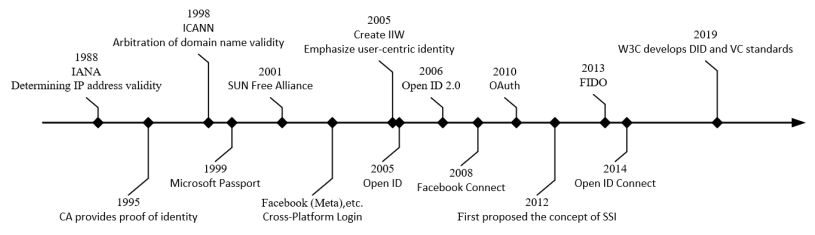
\includegraphics[width=1\textwidth]{Images/c3_1.png} 
  \caption{The timeline of digital identity development.}
\end{figure}

\section{Shifting Identity Paradigms}

This section focuses on the evolution of \gls{idm} models, which have been categorized into three main paradigms. These paradigms describe the evolution of digital identity 
management which show trends for more user-friendly and secure approach.

\renewcommand{\arraystretch}{1.2}
\begin{table}[h]
  \centering
  \small
  \begin{tabular}{|>{\centering\arraybackslash}m{1.8cm}|>{\centering\arraybackslash}m{2.1cm}|>{\centering\arraybackslash}m{1.9cm}|>{\centering\arraybackslash}m{2.2cm}|>{\centering\arraybackslash}m{2.3cm}|>{\centering\arraybackslash}m{2.1cm}|}
    \hline
    \thead{Model \\ Name} & \thead{Credentials \\ Ownership \\ of User} & \thead{Optional \\ Disclosure}  & \thead{Information \\ Silo} & \thead{Support \\ Pseudonyms} & \thead{Centralized \\ Storage}  \\
    \hline
    Centralized Identity & X & X & X & X & V \\
    \hline
    Federated Identity & X & X & V & X & V \\
    \hline
    Self-Sovereign Identity & V & V & X & V & X \\
    \hline
  \end{tabular}
  \caption{Comparison of the characteristics of three models.}
\end{table}

Centralized \gls{idm} model (\gls{idm} 1.0), includes organizations issuing credentials to users, using shared secrets, such as usernames and passwords, for authentication. 
Federated \gls{idm} model (\gls{idm} 2.0) brings in third-party \gls{idp} for \gls{sso} and so still centralizes user's personal identifiable information. Finally, 
Self-Sovereign \gls{idm} model (\gls{idm} 3.0) allows users to have absolute mastery over their digital identities via Digital Wallets using standards such as 
\gls{vc} and \gls{did} \cite{9272212}.

\subsection{Pitfalls of Centralized Identity}

Centralized \gls{idm} models were predominant in the initial stage of the digital identity development process, and these models were managed by 
organizations and institutions. Under this model, people literally gave their personal data to these centralized authoritative bodies, that in return gave them status or 
official recognition \cite{9695553}. Having all personal data in one place was a big plus; on the other hand, it also had some disadvantages.

\begin{figure}[h]  
  \centering
  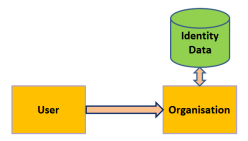
\includegraphics[width=0.5\textwidth]{Images/c3_2.png} 
  \caption{Centralized Identity Management Model (IDM 1.0)}
\end{figure}

One of the primary issues with Centralized \gls{idm} models is that they are naturally prone to security breaches. The fact that all user data were stored in a single 
location meant that in case of a breach in the system, victims of this breach would be subject to widespread data leaks and identity theft \cite{businessreporter}. 
Furthermore, users had to deal with the bother of having too many account names and passwords for the different platforms which increased the risks of password-related 
security issues. Even though it was convenient at first, centralized identity model has proved to be inadequate in helping to solve emerging security threats and 
protecting user privacy.

\subsection{Emergence of Federated Identity}

To deal with the issues caused by the Centralized \gls{idm} models, the idea of the Federated \gls{idm} models appeared, which is much more flexible and user-centered 
\cite{9695553}. These identity management solutions paved the way for \gls{idp}, a system which enables the creation, handling, and implementation of online 
identities.  of federated identities, the users could use a unique identity registered with an \gls{idp} to access different network applications within their
domain, and the authentication process would be simplified to just clicking once.

\begin{figure}[h]  
  \centering
  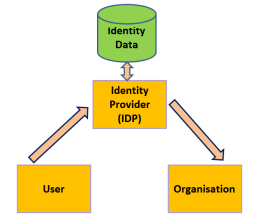
\includegraphics[width=0.5\textwidth]{Images/c3_3.png} 
  \caption{Federated Identity Management Model (IDM 2.0)}
\end{figure}

With the adoption of federated identity solution, user convenience and inter-platform operability have been enhanced, but new security challenges also arise. An expansion
of the \gls{idp} gave rise to a more vulnerable attack surface for Federated \gls{idm} models that made them more prone to data breaches and cyber-attacks \cite{9695553}. 
Furthermore, the usage of several \gls{idp} suggested the possibility of privacy and user consent problems, as the user’s identity information was spread across multiple 
service providers. Federated \gls{idm} models persisted in gaining popularity even though they encountered many challenges owing to their flexibility and ease of use.

\subsection{Evolution towards User-Centric Identity}

In direct response to the rapidly developing issues surrounding traditional Centralized and Federated \gls{idm}s, user-centric identity appeared as a concept, which 
aims to give users back control over their digital identities. Specifically, the so-called Self-Sovereign \gls{idm} models have emphasized the importance of user 
control and consent in identity management, allowing them to store authenticators and certificates issued by a range of service providers in their personal 
devices \cite{9881610}.

\begin{figure}[h]  
  \centering
  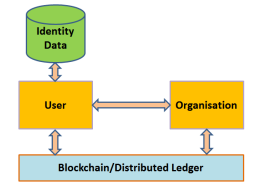
\includegraphics[width=0.5\textwidth]{Images/c3_4.png} 
  \caption{Self-Sovereign Identity Management Model (IDM 3.0)}
\end{figure}

The introduction of blockchain technology was a pivotal transformations in user-centric identity and it provides a decentralized and immutable ledger for identity 
verification. The \gls{ssi} model was based on blockchain that enabled users to retain authority over their data, discarding intermediaries and centralized authorities 
\cite{9881610}. In the \gls{ssi} model, users can securely and privately own and control data and identity information while sharing them in a way, that protects 
their data sovereignty. Eventually, the deployment of \gls{ssi} will need to be fully developed and adopted, however, it constitutes a major milestone on the way to a more 
secure and user-centric model for identity management.